\documentclass[12pt]{article}
\usepackage[left=1cm, right=1cm, top=2cm,bottom=1.5cm]{geometry} 

\usepackage[parfill]{parskip}
\usepackage[utf8]{inputenc}
\usepackage[T2A]{fontenc}
\usepackage[russian]{babel}
\usepackage{enumitem}
\usepackage[normalem]{ulem}
\usepackage{amsfonts, amsmath, amsthm, amssymb, mathtools}

\usepackage{fancyhdr}
\pagestyle{fancy}
\renewcommand{\headrulewidth}{1.5pt}
\renewcommand{\footrulewidth}{1pt}

\usepackage{graphicx}
\usepackage[figurename=Рис.]{caption}
\usepackage{subcaption}
\usepackage{float}

%%Наименование папки откуда забирать изображения
\graphicspath{ {./images/} }

%%Изменение формата для ввода доказательства
\renewcommand{\proofname}{$\square$  \nopunct}
\renewcommand\qedsymbol{$\blacksquare$}

\addto\captionsrussian{%
	\renewcommand{\proofname}{$\square$ \nopunct}%
}
%% Римские цифры
\newcommand{\RN}[1]{%
	\textup{\uppercase\expandafter{\romannumeral#1}}%
}

\theoremstyle{definition}
\newtheorem{defn}{Опр:}
\newtheorem{rem}{Rm:}
\newtheorem{prop}{Утв.}
\newtheorem{exrc}{Упр.}
\newtheorem{lemma}{Лемма}
\newtheorem{theorem}{Теорема}
\newtheorem{corollary}{Следствие}
\newtheorem{axiom}{Аксиома}
\newtheorem*{axiom*}{Аксиома}
\newenvironment{cusdefn}[1]
{\renewcommand\thedefn{#1}\defn}
{\enddefn}

\DeclareRobustCommand{\divby}{%
	\mathrel{\text{\vbox{\baselineskip.65ex\lineskiplimit0pt\hbox{.}\hbox{.}\hbox{.}}}}%
}

\newcommand{\smallerrel}[1]{\mathrel{\mathpalette\smallerrelaux{#1}}}
\newcommand{\smallerrelaux}[2]{\raisebox{.1ex}{\scalebox{.75}{$#1#2$}}}
\newcommand{\smallin}{\smallerrel{\in}}
\newcommand{\smallnotin}{\smallerrel{\notin}}


\begin{document}
	\lhead{Математический анализ - I}
	\chead{Шапошников С.В.}
	\rhead{Лекция - 7}

\begin{theorem}\textbf{(Принцип полноты Вейрштрасса)}:
	Если $A \neq \varnothing$ и ограниченно сверху, то $\exists \sup{A}$.
	Если $A \neq \varnothing$ и ограниченно снизу, то $\exists \inf{A}$.
\end{theorem}
Доказательство смотри в прошлой лекции.

\subsection*{Аксиома Архимеда} 

Для нас \uline{аксиома Архимеда} - это теорема, так как она следует из \uline{аксиомы полноты}. Будем доказывать её как теорему.

\textbf{Аксиомы полноты.} Если $A \subset \mathbb{R}, \, A \neq \varnothing$, $B \subset \mathbb{R}, \, B \neq \varnothing$ и ``$A \leq B$'' (то есть $a \leq b, \, \forall a \in A,\, b \in B$), то $\exists c \in \mathbb{R}$, которое разделяет $A$ и $B$, то есть $a \leq c \leq b, \, \forall a \in A,\, b \in B$.

\textbf{Аксиома Архимеда.}	Множество натуральных чисел $\mathbb{N}$ - не ограниченно сверху в $\mathbb{R}$.

\begin{proof}
	Предположим противное, что $\mathbb{N}$ - ограниченно сверху, тогда по принципу полноты Вейрштрасса $\exists \, a = \sup{\mathbb{N}}$. Посмотрим на $a-1 \Rightarrow (a-1) < \sup{\mathbb{N}} \Rightarrow (a-1)$ - не является верхней гранью $\Rightarrow$ \\
	$\exists \, n \in \mathbb{N} \colon (a-1) < n$. Добавляем 1 справа и слева, получаем $a < n+1$ - противоречит тому, что $a = \sup{\mathbb{N}}$.
\end{proof}

\begin{corollary}
	Если $0 < a < b \Rightarrow \exists \, n\in \mathbb{N} \colon an = b$
\end{corollary}
\begin{proof}
	Поделим на $a \Rightarrow n > \dfrac{b}{a} \Rightarrow$ по аксиоме Архимеда такое $n$ найдется всегда, так как множество не ограниченно.
\end{proof}

\subsection*{Применение Аксиомы Архимеда}
Когда говорим про вещественные числа - используем геометрическую модель. Будем изображать вещественные числа в виде прямой.

\begin{defn}
	\uwave{Прямая} - геометрическое место точек, равноудаленное от двух данных.
\end{defn}

Как построить соответствие между вещественными числами и точкой на прямой?
Надо выбрать начало координат, единичный отрезок. Возьмем вещественное число $a$. В $a$ сколько-то раз умещается едениц. То есть по аксиоме Архимеда $\exists \, n\colon n \leq a < n+1$.

\begin{figure}[H]
	\centering
	\includegraphics[width=0.4\textwidth]{7_1.eps}
	\caption{Соответствие между прямой и точками}
	\label{fig:7_1}
\end{figure}

Далее берем отрезок от 0 до 1 и делим на 10, опять $\exists m\colon \frac{m}{10} \leq a < \frac{m+1}{10}$, $\dotsc$.\\
Таким образом можно отождествить то что делается на прямой с десятичными дробями: $a_0{,}a_1a_2\dotsc$ и так выписать для каждой точки десятичную дробь и наоборот. То есть аксиома Архимеда позволяет измерять отрезки и указывает процедуру сопоставления точек прямой и вещественных чисел.
 
\begin{defn}
 	\uwave{Отрезок} $[a,b] = \{\,x \in \mathbb{R} \colon a\leq x \leq b\,\}$
\end{defn}
\begin{defn}
	\uwave{Интервал} $(a,b) = \{\,x \in \mathbb{R} \colon a < x < b\,\}$
\end{defn}
\begin{defn}
	\uwave{Полуинтервал} $(a,b] = \{\,x \in \mathbb{R} \colon a < x \leq b\,\}$
\end{defn}
\begin{defn}
	\uwave{Полуинтервал} $[a,b) = \{\, \in \mathbb{R} \colon a\leq x < b\,\}$
\end{defn}
\begin{defn}
	\uwave{Модуль} $|x| = \max\{x, -x\}$
\end{defn}

Можно проверить, что $|x-y| = \begin{cases} 
	x-y, & x \geq y\\
	y-x, & x < y
\end{cases}$

\begin{defn}
	Величина $|x-y|$  называется \uwave{расстоянием} от $x$ до $y$. А для отрезков, интервалов, полуинтервалов с концами $\{a, b\}$ число $b-a$ называется \uwave{длиной интервала}. 
\end{defn}

\begin{prop}\textbf{Неравенство треугольника}:
	$\big||x| - |y| \big| \leq |x \pm y| \leq |x| + |y|$
\end{prop}

\begin{proof}
	Поскольку $|x| = \max\{x, -x\}$, то $\pm x \leq |x| \Rightarrow$
	$$ x + y \leq |x| + y \leq |x| + |y|$$
	$$ -x - y \leq |x| - y \leq |x| + |y|$$
Таким образом получим: $|x + y| \leq |x| + |y|$, аналогично
	$$ x - y \leq |x| - y \leq |x| + |y|$$
	$$ -x + y \leq |x| + y \leq |x| + |y|$$
Таким образом получим: $|x - y| \leq |x| + |y| \Rightarrow |x \pm y| \leq |x| +|y|$.

$$ |x + y - x| = |y| \leq |x| + |y - x| \Rightarrow |y| - |x| \leq |y-x|$$
$$ |y + x - y| = |x| \leq |y| + |x - y| \Rightarrow |x| - |y| \leq |x-y| = |y-x|$$
Таким образом получим: $\big||x| - |y|\big| \leq |x - y|$, аналогично
$$ |x - (y + x)| = |-y| = |y| \leq |x| + |y + x| \Rightarrow |y| - |x| \leq |y + x|$$
$$ |y - (x + y)| = |-x| = |x| \leq |y| + |x + y| \Rightarrow |x| - |y| \leq |x + y|$$

Таким образом получим: $\big||x| - |y|\big| \leq |x \pm y|$.

\end{proof}

\begin{defn}
	\uwave{Последовательность} элементов множества $A$ - это функция $f \colon \mathbb{N} \rightarrow A$. Только вместо записи $f(n)$ пишем $a_n$.
\end{defn}

\begin{theorem}\textbf{Принцип полноты Кантора (теорема о вложенных отрезках)}:
	Пусть $[a_1,b_1] \supset [a_2,b_2] \supset \dotsc \supset[a_n,b_n] \supset [a_{n+1}, b_{n+1}] \supset \dotsc$ - последовательность (не строго) вложенных отрезков. Тогда:
	\begin{enumerate}
		\item $\bigcap\limits_{n} [a_n, b_n] \neq \varnothing$;
		\item Если $\forall \varepsilon >0, \, \exists\, n \colon b_n - a_n < \varepsilon \Rightarrow \bigcap\limits_{n} [a_n, b_n] $ - состоит ровно из одной точки;
	\end{enumerate}
\end{theorem}
\begin{proof}
	Выводим из принципа полноты Вейрштрасса:
	$A = \{a_n\}$ - множество левых концов, любой правый конец $b_n$ - является верхней гранью $A$.
	Предположим противное: $\exists \, b_m \colon b_m < a_n$
	
	\begin{figure}[H]
		\centering
		\includegraphics[width=0.34\textwidth]{7_2.eps}
	 	\caption{Непересекающиеся отрезки}
		\label{fig:7_2}
	\end{figure}
	
	Тогда мы получим непересекающиеся отрезки $[a_m, b_m]$ и $[a_n,b_n]$, а это противоречит вложенности. Следовательно, все $a_n$ могут быть только меньше  или равны $b_m$. Так как $A$ - не пусто, ограниченно сверху $\Rightarrow$ по принципу полноты Вейрштрасса $\exists \, c = \sup {A}$. 
	По определению точной верхней грани: $\forall m, c \leq b_m$. По определению верхней грани $\forall n, a_n \leq c \Rightarrow \forall n, m, \, a_n \leq c \leq b_m$. В частности для случая, когда $m =n \Rightarrow \forall n, c \in [a_n, b_n] \Rightarrow$ 1 - доказано. 
	
	Пусть $\exists \, c_1, c_2$ удовлетворяющие условиям выше, но тогда обе эти точки лежат в каждом отрезке $[a_n, b_n]$.
	 \begin{figure}[H]
	 	\centering
	 	\includegraphics[width=0.34\textwidth]{7_3.eps}
	 	\caption{}
	 	\label{fig:7_3}
	 \end{figure}
	Это означает, что $b_n - a_n \geq c_2 - c_1$, но согласно второму пункту для $\varepsilon =\dfrac{c_2 - c_1}{2}$ нет такого отрезка $[a_n,b_n] \Rightarrow$ противоречие $\Rightarrow$ 2 - доказано.
\end{proof}

\begin{corollary}
	$a < b \Rightarrow [a,b]$ - не является счетным множеством.
\end{corollary}

\begin{proof}
	(От противного): пусть $[a,b]$ - счетно и $x_1, x_2, \dotsc, x_n, \dotsc $ - все его элементы. Делим отрезок на три части и берем тот, где нет $x_1$. Затем этот отрезок делим на три части и берем тот, где нет $x_2$. Затем этот отрезок делим на три части и берем тот, где нет $x_3$, $\dotsc$ и так далее $\Rightarrow$ получили систему вложенных отрезков.
	
 	\begin{figure}[H]
		\centering
		\includegraphics[width=0.8\textwidth]{7_4.eps}
	 	\caption{Система вложенных отрезков}
		\label{fig:7_4}
	\end{figure}
	
	По теореме Кантора внутри $\exists \, c$, какой номер у этой точки? Может ли $c = x_n$ - нет, так как на шаге $n$ взяли отрезок в котором нет $x_n \Rightarrow$ такая точка не была пересчитана $\Rightarrow$ противоречие.
\end{proof}
\begin{exrc}
	$a < b$, доказать, что $[a,b] \sim [a,b) \sim (a,b) \sim \mathbb{R}$ (множества равномощны).
\end{exrc}

\begin{defn}
	Множества равномощные отрезку $[a,b]$ с $a < b$ или $\mathbb{R}$ называются \uwave{континуальными}.
\end{defn}

\begin{rem}
	Из принципа \uline{полноты Кантора} и \uline{аксиомы Архимеда} следует \uline{аксиома полноты}. (Доказать как упражнение).
\end{rem}

\section*{Предел последовательности}

Пусть $\{a_n\}$ - последовательность вещественных чисел.

\begin{defn}
	Число $a$ называется \uwave{пределом последовательности} $\{a_n\}$ при $n \rightarrow \infty$, если $$\forall \varepsilon > 0,\, \exists\, N \in \mathbb{N} \colon \forall n > N, \, |a_n - a| < \varepsilon$$
	Обозначение: $\lim\limits_{n \rightarrow \infty}{a_n} = a$, или $a_n \xrightarrow[n\to \infty]{} a$, или просто $a_n \to a$.
\end{defn}

\subsection*{Примеры}
\begin{enumerate}

\item $\lim\limits_{n \rightarrow \infty}{\dfrac{1}{n}} = 0$

 	\begin{figure}[H]
		\centering
		\includegraphics[width=0.5\textwidth]{7_5.eps}
		\caption{Предел последовательности $\frac{1}{n}$}
		\label{fig:7_5}
	\end{figure}

Формально, нужно проверить, что $\forall \varepsilon > 0,\, \exists \, N \in \mathbb{N} \colon \forall n > N, \, |\frac{1}{n} - 0| < \varepsilon$, какое $N$ взять? $\frac{1}{n} < \varepsilon \Rightarrow n > \frac{1}{\varepsilon}$. Подойдет $N > \frac{1}{\varepsilon}$ - такое $N$ найдется по аксиоме Архимеда.

\item $\lim\limits_{n \rightarrow \infty}{\dfrac{1\,}{2^n}} = 0$

Формально, нужно проверить, что $\forall \varepsilon > 0,\, \exists \,N \in \mathbb{N} \colon \forall n > N, \, |\frac{1\,}{2^n} - 0| < \varepsilon$, значит $2^n > \frac{1}{\varepsilon}$.

 По неравенству Бернулли $2^n = (1+1)^n \geq 1+n$. Подойдет $N >  \frac{1}{\varepsilon}$ и для $n > N \Rightarrow 2^n \geq n+1 > N > \frac{1}{\varepsilon}$ - такое $N$ найдется по аксиоме Архимеда.
\end{enumerate}

\subsection*{Отрицание предела последовательности}
Число $a$ не является пределом последовательности $\{a_n\}$? Построим отрицание определения:

\begin{cusdefn}{10}
 $\forall \varepsilon > 0,\, \exists \, N\in \mathbb{N} \colon \forall n > N, \, |a_n - a| < \varepsilon$
\end{cusdefn}
Тогда отрицание: $$\exists\, \varepsilon > 0,\, \forall N \in \mathbb{N} \colon \exists\, n > N\colon |a_n - a| \geq \varepsilon$$

\begin{prop}
	Следующие утверждения эквивалентны:
	\begin{enumerate}[label={\arabic*)}]
		\item $\lim\limits_{n \rightarrow \infty}{a_n} = a$;
		\item Для всякого интервала, содержащего $a$, в нем лежат все члены последовательности, начиная с некоторого номера $N \Leftrightarrow \forall (\alpha,\beta) \ni a, \, \exists \, N \colon \forall n > N, \, a_n \in (\alpha, \beta)$;
		\item Во всяком интервале, содержащим $a$, лежат все члены последовательности, кроме конечного числа $\Leftrightarrow \forall (\alpha,\beta) \ni a, \, \exists \, n_1, \dotsc, n_N \colon a_n \in (\alpha,\beta), \, \forall n \notin \{n_1, \dotsc, n_N\}$;
	\end{enumerate}
\end{prop}

\begin{proof}
Докажем утверждения циклично:\\
$1) \Rightarrow 2)$\\
  $\forall \varepsilon > 0,\, \exists \, N \in \mathbb{N} \colon \forall n > N, \, |a_n - a| < \varepsilon \Leftrightarrow a_n \in (a - \varepsilon, a + \varepsilon)$ начиная с некоторого номера $n$. Пусть $a \in (\alpha, \beta) \Rightarrow \varepsilon = \min\{a - \alpha,\beta - a\} \Rightarrow$ возьмем наименьший симметричный интервал внутри $(\alpha, \beta)$. По пункту 1) следует $\exists \, N\colon \, \forall n > N,\, a_n \in (a-\varepsilon, a + \varepsilon) \subset (\alpha,\beta)$.
  
$2) \Rightarrow 3)$\\ 
  $\forall (\alpha,\beta) \ni a, \, \exists \, N \colon \forall n > N, \, a_n \in (\alpha, \beta) \Rightarrow a_n \notin (\alpha, \beta)$ возможно только для $n \in \{1,\dotsc,N\}$.
  
$3) \Rightarrow 1)$\\ 
	$\forall \varepsilon > 0$ рассмотрим интервал $(a - \varepsilon, a + \varepsilon)$. По пункту 3) $\exists n_1, \dotsc ,n_N \colon \forall n \notin \{n_1,\dotsc,n_N\}, \, a_n \in (a - \varepsilon, a + \varepsilon)$. Возьмем $\tilde{N} = \max \{n_1,\dotsc,n_N\}$, тогда $\forall n > \tilde{N}, 
	\, n \notin \{n_1,\dotsc,n_N\} \Rightarrow a_n \in (a - \varepsilon, a + \varepsilon) \Leftrightarrow |a_n - a| < \varepsilon$.
\end{proof}

\begin{corollary}
	Отбрасывание или добавление конечного числа элементов - не влияет на сходимость и значения предела последовательности (по 3-му свойству).
\end{corollary}


\begin{theorem}
	У последовательности число пределов $\leq 1$.
\end{theorem}

\begin{proof}
	Предположим, что $\lim\limits_{n \rightarrow \infty}{a_n} = a$ и $\lim\limits_{n \rightarrow \infty}{a_n} = b$ такие, что $a \neq b$. Для определенности пусть $a < b$. Тогда рисуем прямую и берем два непересекающихся интервала:
	
 	\begin{figure}[H]
		\centering
		\includegraphics[width=0.3\textwidth]{7_6.eps}
		\caption{Разные пределы последовательностей}
		\label{fig:7_6}
	\end{figure}
	
Берем $0 < \varepsilon < \frac{b-a}{2}$ - чтобы точно не пересекались. Тогда $\exists \, N_1 \colon \, \forall n > N_1, \, a_n \in I_a$, $\exists \, N_2 \colon \, \forall n > N_2, \, a_n \in I_b$.\\
Пусть $n > \max \{N_1, N_2\} \Rightarrow a_n \in I_a \cap I_b = \varnothing \Rightarrow$ противоречие. Значит предел определен единственным образом.
\end{proof}

\end{document}